%&tex
\documentclass{standalone}

\usepackage[dvipsnames]{xcolor}

\usepackage{tikz}
\usetikzlibrary{positioning}
\usepackage{bm}
\usepackage{amsmath}
\usepackage{amsfonts}

\begin{document}

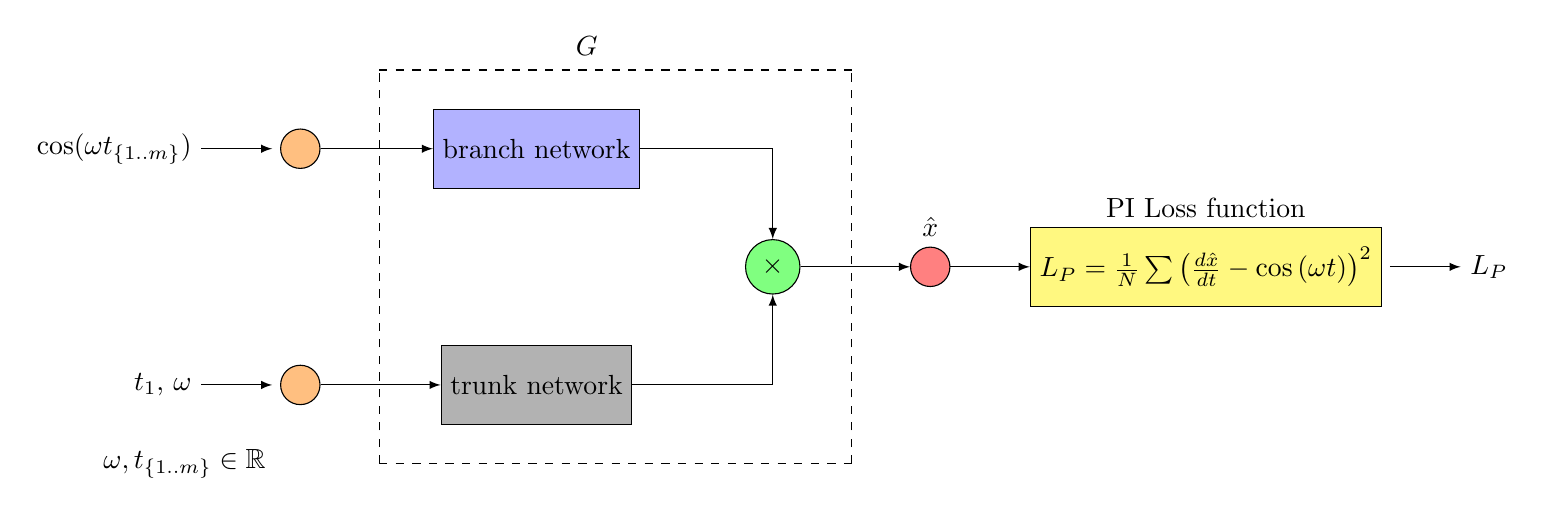
\begin{tikzpicture}

    % branch input node
    \node[draw,
    circle,
    minimum size = 0.5cm,
    fill = orange!50](BR_input) at (0, 3){};

    % trunk input node
    \node[draw,
    circle,
    minimum size = 0.5cm,
    fill = orange!50](TR_input) at (0,0) {};

    % branch network
    \node[draw,
    rectangle,
    minimum width = 2cm,
    minimum height = 1cm,
    fill = blue!30](BR_net) at (3,3) {branch network};

    % trunk network
    \node[draw,
    rectangle,
    minimum width = 2cm,
    minimum height = 1cm,
    fill = black!30](TR_net) at (3,0) {trunk network};

    % dot product node
    \node[draw,
    circle,
    minimum size = 0.5cm,
    fill = green!50](dot) at (6,1.5) {\(\times\)};

    % output node
    \node[draw,
    circle,
    minimum size = 0.5cm,
    label = \(\hat{x}\),
    fill = red!50](Output) at (8,1.5) {};

    % PI function node
    \node[draw,
    rectangle,
    minimum width = 1.0cm,
    minimum height = 1.0cm,
    label = PI Loss function,
    fill = yellow!50](PIfunction) at (11.5,1.5) {\( L_P = \frac{1}{N} \sum \left(\frac{d \hat{x}}{dt} - \cos\left(\omega t\right) \right)^2\)};

    \draw[dashed] (1,-1) -- (7,-1);
    \draw[dashed] (1,-1) -- (1,4);
    \draw[dashed] (7,-1) -- (7,4);
    \draw[dashed] (1,4) -- (7,4);
    \node[text width = 1cm] at (4.0,4.3) {\(G\)};

    \node[text width = 5cm] at (0,-1) {\(\omega,t_{\{1..m\}} \in \mathbb{R}\)};

    \draw[-latex] (BR_input.east) -- (BR_net);
    \draw[-latex] (TR_input.east) -- (TR_net);
    \draw[-latex] (TR_net.east) -| (dot);
    \draw[-latex] (BR_net.east) -| (dot);
    \draw[-latex] (dot.east) -- (Output.west);
    \draw[-latex] (Output.east) -- (PIfunction.west);

    % labeling inputs and outputs
    \draw[latex-, shorten <= 1mm] (BR_input.west) -- ++(-1,0) node[left]{\(\cos(\omega t_{\{1..m\}})\)};
    \draw[latex-, shorten <= 1mm] (TR_input.west) -- ++(-1,0) node[left]{\(t_1\), \(\omega\)};
    \draw[-latex, shorten <= 1mm] (PIfunction.east) -- ++(1,0) node[right]{\(L_P\)};


\end{tikzpicture}

\end{document}
